\documentclass{article}

%========================================================================================
% PREAMBLE
% This section loads all necessary packages and defines the document's overall layout.
%========================================================================================
\usepackage[letterpaper, margin=1in, textwidth=6.5in]{geometry} % Manages page layout (margins, paper size).
\usepackage{graphicx}       % Required for including images (though none are used directly in this text).
\usepackage{amsmath}        % Provides advanced environments for equations (like align*).
\usepackage{amssymb}        % Provides additional mathematical symbols.
\usepackage{amsfonts}       % Provides mathematical fonts.
\usepackage{enumitem}       % Allows for customization of list environments (e.g., adding space between items).
\usepackage{pdfpages}       % Allows for the inclusion of entire pages from external PDF files.
\usepackage{chemformula}    % Simplifies writing chemical formulas (e.g., \ch{H2O}).
\usepackage{siunitx}        % Provides standardized formatting for numbers and units (e.g., \SI{1.00}{g/mol}).
\usepackage{hyperref}       % Creates hyperlinks within the document (useful for navigation in PDF viewers).
\hypersetup{
    colorlinks=true,
    linkcolor=blue,
    filecolor=magenta,      
    urlcolor=cyan,
}

% DOCUMENT METADATA
\title{Comprehensive Study Guide for Chemistry Exam 2}
\author{} % Author and date are left blank as requested.
\date{}

\begin{document}

\maketitle % Generates the title.

%========================================================================================
% CHAPTER 5: IONIC AND COVALENT COMPOUNDS
%========================================================================================
\section*{Chapter 5: Ionic and Covalent Compounds}

\subsection*{Ionic vs. Molecular Compounds}
\begin{itemize}[itemsep=5pt]
    \item \textbf{Ionic Compound:} A compound composed of a \textbf{metal} and a \textbf{nonmetal}. These compounds are formed by the transfer of electrons, creating positively charged ions (cations) and negatively charged ions (anions) held together by electrostatic attraction. Example: NaCl (Sodium is a metal, Chlorine is a nonmetal).
    \item \textbf{Molecular Compound:} A compound composed of only \textbf{nonmetals}. These compounds are formed by the sharing of electrons to form covalent bonds. Example: H\(_2\)O (Hydrogen and Oxygen are both nonmetals).
\end{itemize}

\subsubsection*{Practice Problems: Classification}
\begin{enumerate}[itemsep=5pt]
    \item \textbf{Classify KBr:} Potassium (K) is a Group 1 metal. Bromine (Br) is a Group 17 nonmetal. Since it's a metal + nonmetal, KBr is an \textbf{ionic} compound.
    \item \textbf{Classify P\(_4\)O\(_6\):} Phosphorus (P) is a nonmetal. Oxygen (O) is a nonmetal. Since it's composed of only nonmetals, P\(_4\)O\(_6\) is a \textbf{molecular} compound.
    \item \textbf{Classify Fe(NO\(_3\))\(_3\):} Iron (Fe) is a transition metal. The nitrate ion (NO\(_3^-\)) is a polyatomic ion composed of nonmetals. The bond is between the metal cation Fe\(^{3+}\) and the polyatomic anion NO\(_3^-\). Therefore, it is an \textbf{ionic} compound.
\end{enumerate}

\subsection*{Lattice Energy}
\begin{itemize}[itemsep=5pt]
    \item \textbf{Definition:} Lattice energy is a measure of the stability of an ionic compound. It is the energy required to completely separate one mole of a solid ionic compound into its gaseous ions.
    \item \textbf{Trends:} Lattice energy is governed by Coulomb's Law, which states that the force (and thus energy) is proportional to the charges of the ions and inversely proportional to the distance between them. 
    \[ E \propto \frac{Q_1 \times Q_2}{d} \]
    \begin{itemize}
        \item \textbf{Ionic Charge (Q):} As the magnitude of the charges on the ions increases, the lattice energy \textbf{increases dramatically}. This is the most dominant factor. (e.g., +2/-2 is much stronger than +1/-1).
        \item \textbf{Atomic Radius (d):} As the size of the ions (and thus the distance, d, between them) increases, the lattice energy \textbf{decreases}.
    \end{itemize}
\end{itemize}

\subsubsection*{Practice Problems: Ranking by Lattice Energy}
\begin{enumerate}[itemsep=5pt]
    \item \textbf{Arrange MgO, CaO, and SrO in order of increasing lattice energy.}
    \begin{itemize}
        \item \textbf{Charges:} All compounds have +2 (Mg\(^{2+}\), Ca\(^{2+}\), Sr\(^{2+}\)) and -2 (O\(^{2-}\)) ions. Since charges are the same, we must look at the ionic radius.
        \item \textbf{Radius:} The cation radii increase down the group: Mg\(^{2+}\) < Ca\(^{2+}\) < Sr\(^{2+}\).
        \item \textbf{Conclusion:} Since lattice energy is inversely proportional to radius, the compound with the smallest radius (MgO) will have the highest lattice energy. The order of increasing lattice energy is \textbf{SrO < CaO < MgO}.
    \end{itemize}
    \item \textbf{Arrange NaCl, MgI\(_2\), and AlN in order of increasing lattice energy.}
    \begin{itemize}
        \item \textbf{Charges:} We evaluate the magnitude of the charges first.
        \begin{itemize}
            \item NaCl: Na\(^{+}\) and Cl\(^{-}\) (+1, -1)
            \item MgI\(_2\): Mg\(^{2+}\) and I\(^{-}\) (+2, -1)
            \item AlN: Al\(^{3+}\) and N\(^{3-}\) (+3, -3)
        \end{itemize}
        \item \textbf{Conclusion:} The product of the charges increases significantly: NaCl (1x1=1) < MgI\(_2\) (2x1=2) < AlN (3x3=9). Therefore, the order of increasing lattice energy is \textbf{NaCl < MgI\(_2\) < AlN}.
    \end{itemize}
     \item \textbf{Arrange LiF, KBr, and MgO in order of increasing lattice energy.}
    \begin{itemize}
        \item \textbf{Charges:} LiF (+1, -1), KBr (+1, -1), MgO (+2, -2). The charge magnitude is the dominant factor. MgO will have the highest lattice energy by a large margin.
        \item \textbf{Radius (for LiF vs KBr):} K\(^+\) is larger than Li\(^+\), and Br\(^-\) is larger than F\(^-\). Therefore, the distance between ions in KBr is significantly larger than in LiF. This means LiF has a higher lattice energy than KBr.
        \item \textbf{Conclusion:} The final order of increasing lattice energy is \textbf{KBr < LiF < MgO}.
    \end{itemize}
\end{enumerate}

\subsection*{Nomenclature}
\subsubsection*{Items to Memorize for Nomenclature}
\begin{enumerate}[itemsep=5pt]
    \item \textbf{Common Ionic Charges:} From \textbf{slide 9 of "Chapter 5 Ionic and Covalent Compounds.pdf"}:
    \begin{itemize}
        \item Group 1: +1
        \item Group 2: +2
        \item Group 13: +3 (for Al, Ga)
        \item Group 15: -3
        \item Group 16: -2
        \item Group 17: -1
    \end{itemize}
    \item \textbf{Molecular Prefixes:} From \textbf{slide 23 of "Chapter 5 Ionic and Covalent Compounds.pdf"}:
    \begin{itemize}
        \item 1: mono- \quad 2: di- \quad 3: tri- \quad 4: tetra- \quad 5: penta-
        \item 6: hexa- \quad 7: hepta- \quad 8: octa- \quad 9: nona- \quad 10: deca-
    \end{itemize}
    \item \textbf{Polyatomic Ions:} From \textbf{slide 36 of "Chapter 5 Ionic and Covalent Compounds.pdf"}:
    \begin{itemize}
        \item Acetate: C\(_2\)H\(_3\)O\(_2^-\) \quad Carbonate: CO\(_3^{2-}\) \quad Hydroxide: OH\(^-\) \quad Nitrite: NO\(_2^-\)
        \item Nitrate: NO\(_3^-\) \quad Chromate: CrO\(_4^{2-}\) \quad Dichromate: Cr\(_2\)O\(_7^{2-}\) \quad Phosphate: PO\(_4^{3-}\)
        \item Ammonium: NH\(_4^+\) \quad Hypochlorite: ClO\(^-\) \quad Chlorite: ClO\(_2^-\) \quad Chlorate: ClO\(_3^-\)
        \item Perchlorate: ClO\(_4^-\) \quad Permanganate: MnO\(_4^-\) \quad Sulfite: SO\(_3^{2-}\) \quad Sulfate: SO\(_4^{2-}\)
        \item Cyanide: CN\(^-\) \quad Peroxide: O\(_2^{2-}\)
    \end{itemize}
\end{enumerate}

\subsubsection*{Practice Problems: Nomenclature}
\begin{enumerate}[itemsep=5pt]
    \item \textbf{Name the compound Fe\(_2\)(SO\(_4\))\(_3\).}
    \begin{itemize}
        \item \textbf{Type:} Ionic (Fe is a metal, SO\(_4^{2-}\) is a polyatomic anion).
        \item \textbf{Anion:} SO\(_4^{2-}\) is the \textbf{sulfate} ion.
        \item \textbf{Cation Charge:} There are 3 sulfate ions, each with a -2 charge, for a total negative charge of \(3 \times (-2) = -6\). To balance this, the two iron ions must have a total positive charge of +6. Therefore, each iron ion is Fe\(^{3+}\).
        \item \textbf{Name:} Iron is a transition metal, so we use a Roman numeral. The name is \textbf{Iron (III) sulfate}.
    \end{itemize}
    \item \textbf{Write the formula for tetraphosphorus decoxide.}
    \begin{itemize}
        \item \textbf{Type:} Molecular (phosphorus and oxygen are nonmetals). The prefixes tell us the number of atoms.
        \item \textbf{Prefixes:} "tetra-" means 4. "deca-" means 10.
        \item \textbf{Formula:} 4 Phosphorus atoms (P\(_4\)) and 10 Oxygen atoms (O\(_{10}\)). The formula is \textbf{P\(_4\)O\(_{10}\)}.
    \end{itemize}
    \item \textbf{Name the acid H\(_2\)SO\(_3\).}
    \begin{itemize}
        \item \textbf{Type:} Oxoacid (contains H, O, and another nonmetal).
        \item \textbf{Identify Anion:} The anion is SO\(_3^{2-}\), which is the \textbf{sulfite} ion.
        \item \textbf{Rule:} Acids from anions ending in "-ite" are named with the suffix "-ous acid".
        \item \textbf{Name:} The name is \textbf{Sulfurous acid}.
    \end{itemize}
\end{enumerate}

\subsection*{Empirical and Molecular Formulas}
\begin{itemize}[itemsep=5pt]
    \item \textbf{Empirical Formula:} The simplest whole-number ratio of atoms of each element present in a compound.
    \item \textbf{Molecular Formula:} The actual number of atoms of each element in a molecule. It is a whole-number multiple of the empirical formula.
\end{itemize}

\subsubsection*{Practice Problems: Formulas}
\begin{enumerate}[itemsep=5pt]
    \item \textbf{The molecular formula for glucose is C\(_6\)H\(_{12}\)O\(_6\). What is its empirical formula?}
    \begin{itemize}
        \item \textbf{Ratio:} The subscripts are 6, 12, and 6.
        \item \textbf{Simplify:} The greatest common divisor is 6. Divide all subscripts by 6: \( \frac{6}{6}=1, \frac{12}{6}=2, \frac{6}{6}=1 \).
        \item \textbf{Answer:} The empirical formula is \textbf{CH\(_2\)O}.
    \end{itemize}
    \item \textbf{A compound has an empirical formula of NO\(_2\) and a molar mass of \SI{92.02}{g/mol}. What is its molecular formula?}
    \begin{itemize}
        \item \textbf{Empirical Mass:} The mass of NO\(_2\) is \(14.01 + 2(16.00) = \SI{46.01}{g/mol}\).
        \item \textbf{Find Multiplier:} Divide the molecular mass by the empirical mass: \( \frac{\SI{92.02}{g/mol}}{\SI{46.01}{g/mol}} \approx 2 \).
        \item \textbf{Molecular Formula:} Multiply the subscripts in the empirical formula by the multiplier (2): N\(_{1 \times 2}\)O\(_{2 \times 2}\) = \textbf{N\(_2\)O\(_4\)}.
    \end{itemize}
    \item \textbf{The molecular formula for octane is C\(_8\)H\(_{18}\). What is its empirical formula?}
     \begin{itemize}
        \item \textbf{Ratio:} The subscripts are 8 and 18.
        \item \textbf{Simplify:} The greatest common divisor is 2. Divide both by 2: \( \frac{8}{2}=4, \frac{18}{2}=9 \).
        \item \textbf{Answer:} The empirical formula is \textbf{C\(_4\)H\(_9\)}.
    \end{itemize}
\end{enumerate}

\bigskip

%========================================================================================
% CHAPTER 8: CHEMICAL REACTIONS
%========================================================================================
\section*{Chapter 8: Chemical Reactions}

\subsection*{Balancing Equations and Reaction Types}
\begin{itemize}[itemsep=5pt]
    \item \textbf{Balancing:} Chemical equations must be balanced to satisfy the Law of Conservation of Mass. The number of atoms of each element must be identical on both the reactant and product sides. This is achieved by adjusting the stoichiometric coefficients.
    \item \textbf{Reaction Types:}
    \begin{itemize}
        \item \textbf{Synthesis (Combination):} Two or more reactants combine to form a single product. (A + B \(\rightarrow\) AB)
        \item \textbf{Decomposition:} A single compound breaks down into two or more simpler substances. (AB \(\rightarrow\) A + B)
        \item \textbf{Single Replacement:} An element replaces another element in a compound. (A + BC \(\rightarrow\) AC + B)
        \item \textbf{Double Replacement:} The cations and anions of two ionic compounds switch places. (AB + CD \(\rightarrow\) AD + CB)
        \item \textbf{Combustion:} A substance (often a hydrocarbon) reacts rapidly with oxygen (O\(_2\)) to produce heat and light. Complete combustion of a hydrocarbon produces CO\(_2\) and H\(_2\)O.
    \end{itemize}
\end{itemize}

\subsubsection*{Practice Problems: Balancing and Classification}
\begin{enumerate}[itemsep=5pt]
    \item \textbf{Balance and classify: \_\_Fe\(_2\)O\(_3\)(s) + \_\_C(s) \(\rightarrow\) \_\_Fe(s) + \_\_CO\(_2\)(g)}
    \begin{itemize}
        \item \textbf{Balance:} Start with Fe. Place a 2 in front of Fe. Now balance O by placing a 3 in front of CO\(_2\). This gives 6 O atoms. Place a 3 in front of C to balance the carbon atoms. Wait, the oxygens in CO2 give 6 O atoms, but there are 3 on the left. Let's restart. Let's put a 2 in front of Fe\(_2\)O\(_3\). That gives 4 Fe and 6 O. So we put a 4 in front of Fe. To get 6 O, we put a 3 in front of CO\(_2\). This requires 3 C.
        \item \textbf{Balanced Equation:} \textbf{2 Fe\(_2\)O\(_3\)(s) + 3 C(s) \(\rightarrow\) 4 Fe(s) + 3 CO\(_2\)(g)}
        \item \textbf{Classification:} Carbon is replacing iron in the oxide compound. This is a \textbf{Single Replacement} reaction.
    \end{itemize}
    \item \textbf{Balance and classify: \_\_C\(_3\)H\(_8\)(g) + \_\_O\(_2\)(g) \(\rightarrow\) \_\_CO\(_2\)(g) + \_\_H\(_2\)O(l)}
    \begin{itemize}
        \item \textbf{Balance:} Balance C first: 3 CO\(_2\). Balance H next: 4 H\(_2\)O. Now count the total oxygen atoms on the right: \(3 \times 2 + 4 \times 1 = 10\). Place a 5 in front of O\(_2\).
        \item \textbf{Balanced Equation:} \textbf{C\(_3\)H\(_8\)(g) + 5 O\(_2\)(g) \(\rightarrow\) 3 CO\(_2\)(g) + 4 H\(_2\)O(l)}
        \item \textbf{Classification:} A hydrocarbon reacts with oxygen. This is a \textbf{Combustion} reaction.
    \end{itemize}
    \item \textbf{Balance and classify: \_\_AgNO\(_3\)(aq) + \_\_Ba(s) \(\rightarrow\) \_\_Ba(NO\(_3\))\(_2\)(aq) + \_\_Ag(s)}
     \begin{itemize}
        \item \textbf{Balance:} There are 2 nitrate groups on the right, so put a 2 in front of AgNO\(_3\). This requires 2 Ag atoms, so put a 2 in front of Ag on the right. Ba is already balanced.
        \item \textbf{Balanced Equation:} \textbf{2 AgNO\(_3\)(aq) + Ba(s) \(\rightarrow\) Ba(NO\(_3\))\(_2\)(aq) + 2 Ag(s)}
        \item \textbf{Classification:} Barium (an element) is replacing silver (an element) in a compound. This is a \textbf{Single Replacement} reaction.
    \end{itemize}
\end{enumerate}

\subsection*{Combustion Analysis}
\textbf{Method:} Use the masses of CO\(_2\) and H\(_2\)O produced from the combustion of a compound to find its empirical formula.
\begin{enumerate}[itemsep=3pt]
    \item Convert mass of CO\(_2\) to moles of C.
    \item Convert mass of H\(_2\)O to moles of H.
    \item If the compound contains oxygen, find the mass of C and H, subtract from the total sample mass to find the mass of O, then convert mass of O to moles of O.
    \item Divide all mole values by the smallest mole value to find the mole ratio (the subscripts for the empirical formula).
    \item If necessary, multiply by a small integer to get whole numbers.
\end{enumerate}

\subsubsection*{Practice Problems: Combustion Analysis}
\begin{enumerate}[itemsep=5pt]
    \item \textbf{Combustion of \SI{18.80}{g} of glucose (C\(_x\)H\(_y\)O\(_z\)) produces \SI{27.6}{g} of CO\(_2\) and \SI{11.3}{g} of H\(_2\)O. Find the empirical formula.}
    \begin{itemize}
        \item \textbf{Moles C:} \( 27.6 \text{ g CO}_2 \times \frac{1 \text{ mol CO}_2}{44.01 \text{ g CO}_2} \times \frac{1 \text{ mol C}}{1 \text{ mol CO}_2} \approx 0.627 \text{ mol C} \)
        \item \textbf{Moles H:} \( 11.3 \text{ g H}_2\text{O} \times \frac{1 \text{ mol H}_2\text{O}}{18.02 \text{ g H}_2\text{O}} \times \frac{2 \text{ mol H}}{1 \text{ mol H}_2\text{O}} \approx 1.254 \text{ mol H} \)
        \item \textbf{Mass C & H:} \( (0.627 \text{ mol C} \times 12.01 \frac{\text{g}}{\text{mol}}) + (1.254 \text{ mol H} \times 1.008 \frac{\text{g}}{\text{mol}}) \approx 7.53 \text{ g C} + 1.26 \text{ g H} = 8.79 \text{ g} \)
        \item \textbf{Mass & Moles O:} Mass O = \(18.80 \text{ g} - 8.79 \text{ g} = 10.01 \text{ g O}\). Moles O = \( 10.01 \text{ g O} \times \frac{1 \text{ mol O}}{16.00 \text{ g O}} \approx 0.626 \text{ mol O} \)
        \item \textbf{Ratio:} Divide by the smallest (0.626): C: \( \frac{0.627}{0.626} \approx 1 \). H: \( \frac{1.254}{0.626} \approx 2 \). O: \( \frac{0.626}{0.626} = 1 \).
        \item \textbf{Answer:} The empirical formula is \textbf{CH\(_2\)O}.
    \end{itemize}
    \item \textbf{A \SI{0.250}{g} sample of a compound containing C, H, and O is combusted to produce \SI{0.568}{g} CO\(_2\) and \SI{0.232}{g} H\(_2\)O. Find the empirical formula.}
    \begin{itemize}
        \item \textbf{Moles C:} \( 0.568 \text{ g CO}_2 \times \frac{1 \text{ mol C}}{44.01 \text{ g CO}_2} \approx 0.0129 \text{ mol C} \)
        \item \textbf{Moles H:} \( 0.232 \text{ g H}_2\text{O} \times \frac{2 \text{ mol H}}{18.02 \text{ g H}_2\text{O}} \approx 0.0257 \text{ mol H} \)
        \item \textbf{Mass C & H:} \( (0.0129 \times 12.01) + (0.0257 \times 1.008) \approx 0.155 \text{ g C} + 0.026 \text{ g H} = 0.181 \text{ g} \)
        \item \textbf{Mass & Moles O:} Mass O = \(0.250 - 0.181 = 0.069 \text{ g O}\). Moles O = \( \frac{0.069}{16.00} \approx 0.00431 \text{ mol O} \)
        \item \textbf{Ratio:} Divide by smallest (0.00431): C: \( \frac{0.0129}{0.00431} \approx 3 \). H: \( \frac{0.0257}{0.00431} \approx 6 \). O: \( \frac{0.00431}{0.00431} = 1 \).
        \item \textbf{Answer:} The empirical formula is \textbf{C\(_3\)H\(_6\)O}.
    \end{itemize}
    \item \textbf{A compound has 48.6\% C, 8.2\% H, and 43.2\% O. Find its empirical formula. If its molar mass is \SI{148.2}{g/mol}, what is the molecular formula?}
    \begin{itemize}
        \item \textbf{Assume 100g sample:} 48.6 g C, 8.2 g H, 43.2 g O.
        \item \textbf{Moles:} C: \( \frac{48.6}{12.01} \approx 4.047 \). H: \( \frac{8.2}{1.008} \approx 8.135 \). O: \( \frac{43.2}{16.00} = 2.700 \).
        \item \textbf{Ratio:} Divide by smallest (2.700): C: \( \frac{4.047}{2.700} \approx 1.5 \). H: \( \frac{8.135}{2.700} \approx 3 \). O: \( \frac{2.700}{2.700} = 1 \).
        \item \textbf{Whole Numbers:} The ratio is 1.5:3:1. Multiply by 2 to clear the decimal: \textbf{3:6:2}.
        \item \textbf{Empirical Formula:} \textbf{C\(_3\)H\(_6\)O\(_2\)}.
        \item \textbf{Molecular Formula:} Empirical mass = \(3(12.01) + 6(1.008) + 2(16.00) = \SI{74.08}{g/mol}\). Multiplier = \( \frac{148.2}{74.08} \approx 2 \).
        \item \textbf{Answer:} The molecular formula is \(2 \times (\text{C}_3\text{H}_6\text{O}_2) = \textbf{C}_6\textbf{H}_{12}\textbf{O}_4\).
    \end{itemize}
\end{enumerate}

\bigskip

%========================================================================================
% CHAPTER 9: AQUEOUS REACTIONS
%========================================================================================
\section*{Chapter 9: Molarity, Dilutions, and Solution Stoichiometry}

\subsection*{Molarity Calculations}
\begin{itemize}[itemsep=5pt]
    \item \textbf{Definition:} Molarity (M) is a unit of concentration, defined as moles of solute per liter of solution.
    \[ M = \frac{\text{moles of solute (n)}}{\text{liters of solution (V)}} \]
\end{itemize}

\subsubsection*{Practice Problems: Molarity}
\begin{enumerate}[itemsep=5pt]
    \item \textbf{Calculate the molarity of a solution made by dissolving 0.50 moles of NaCl in enough water to make a 0.75 L solution.}
    \[ M = \frac{n}{V} = \frac{0.50 \text{ mol}}{0.75 \text{ L}} = \textbf{0.67 M} \]
    \item \textbf{How many grams of CaCl\(_2\) are needed to make \SI{750.0}{mL} of a \SI{0.100}{M} solution?}
    \begin{itemize}
        \item \textbf{Find Moles:} \( n = M \times V = (0.100 \frac{\text{mol}}{\text{L}}) \times (0.7500 \text{ L}) = 0.0750 \text{ mol CaCl}_2 \)
        \item \textbf{Find Grams:} Molar mass of CaCl\(_2\) is \SI{110.98}{g/mol}.
        \[ 0.0750 \text{ mol CaCl}_2 \times \frac{110.98 \text{ g CaCl}_2}{1 \text{ mol CaCl}_2} = \textbf{8.32 g CaCl\(_2\)} \]
    \end{itemize}
    \item \textbf{What volume (in mL) of a \SI{1.50}{M} ethanol solution is needed to provide \SI{4.30}{g} of ethanol (C\(_2\)H\(_5\)OH)?}
     \begin{itemize}
        \item \textbf{Find Moles:} Molar mass of C\(_2\)H\(_5\)OH is \SI{46.07}{g/mol}.
        \[ 4.30 \text{ g} \times \frac{1 \text{ mol}}{46.07 \text{ g}} \approx 0.0933 \text{ mol} \]
        \item \textbf{Find Volume:} \( V = \frac{n}{M} = \frac{0.0933 \text{ mol}}{1.50 \text{ mol/L}} \approx 0.0622 \text{ L} \)
        \item \textbf{Convert to mL:} \( 0.0622 \text{ L} \times 1000 \frac{\text{mL}}{\text{L}} = \textbf{62.2 mL} \)
    \end{itemize}
\end{enumerate}

\subsection*{Dilutions}
\begin{itemize}[itemsep=5pt]
    \item \textbf{Definition:} Dilution is the process of decreasing the concentration of a solution by adding more solvent. The moles of solute remain constant.
    \item \textbf{Formula:} \( M_1V_1 = M_2V_2 \), where M\(_1\) and V\(_1\) are the initial molarity and volume, and M\(_2\) and V\(_2\) are the final molarity and volume.
\end{itemize}

\subsubsection*{Practice Problems: Dilutions}
\begin{enumerate}[itemsep=5pt]
    \item \textbf{To what volume must you dilute \SI{30.0}{mL} of a \SI{12}{M} HCl solution to make a \SI{0.35}{M} solution?}
    \[ M_1V_1 = M_2V_2 \implies V_2 = \frac{M_1V_1}{M_2} = \frac{(12 \text{ M})(30.0 \text{ mL})}{0.35 \text{ M}} \approx \textbf{1.0 \times 10\(_3\)} \text{ mL} \]
    \item \textbf{What volume of a \SI{1.25}{M} KMnO\(_4\) stock solution is needed to prepare \SI{2.50}{L} of a \SI{0.400}{M} solution?}
    \[ V_1 = \frac{M_2V_2}{M_1} = \frac{(0.400 \text{ M})(2.50 \text{ L})}{1.25 \text{ M}} = 0.800 \text{ L} = \textbf{800. mL} \]
    \item \textbf{If \SI{75.0}{mL} of a \SI{0.992}{M} KNO\(_3\) solution is diluted to exactly \SI{250}{mL}, what is the final concentration?}
     \[ M_2 = \frac{M_1V_1}{V_2} = \frac{(0.992 \text{ M})(75.0 \text{ mL})}{250 \text{ mL}} = \textbf{0.298 M} \]
\end{enumerate}

\subsection*{Solution Stoichiometry and Titrations}
\begin{itemize}[itemsep=5pt]
    \item \textbf{Definition:} Using molarity and volume to relate the amounts of reactants and products in a chemical reaction in solution. A \textbf{titration} is a lab technique used to determine an unknown concentration of a solution by reacting it with a solution of known concentration.
\end{itemize}

\subsubsection*{Practice Problems: Titrations}
\begin{enumerate}[itemsep=5pt]
    \item \textbf{What volume (in L) of a \SI{0.203}{M} NaOH solution is needed to neutralize \SI{0.0250}{L} of a \SI{0.188}{M} H\(_2\)SO\(_4\) solution? Reaction: 2 NaOH + H\(_2\)SO\(_4\) \(\rightarrow\) Na\(_2\)SO\(_4\) + 2 H\(_2\)O.}
    \begin{align*}
        \text{Vol NaOH} &= 0.0250 \text{ L H}_2\text{SO}_4 \times \frac{0.188 \text{ mol H}_2\text{SO}_4}{1 \text{ L H}_2\text{SO}_4} \times \frac{2 \text{ mol NaOH}}{1 \text{ mol H}_2\text{SO}_4} \times \frac{1 \text{ L NaOH}}{0.203 \text{ mol NaOH}} \\
        &= \textbf{0.0463 L}
    \end{align*}
    \item \textbf{What is the mass (in grams) of Ag\(_2\)CrO\(_4\) that will precipitate when \SI{150.}{mL} of \SI{0.500}{M} AgNO\(_3\) are added to \SI{100.}{mL} of \SI{0.400}{M} K\(_2\)CrO\(_4\)? Reaction: 2 AgNO\(_3\) + K\(_2\)CrO\(_4\) \(\rightarrow\) Ag\(_2\)CrO\(_4\) + 2 KNO\(_3\).}
    \begin{itemize}
        \item \textbf{This is a limiting reactant problem.}
        \item \textbf{Moles AgNO\(_3\):} \(0.150 \text{ L} \times 0.500 \text{ M} = 0.0750 \text{ mol}\)
        \item \textbf{Moles K\(_2\)CrO\(_4\):} \(0.100 \text{ L} \times 0.400 \text{ M} = 0.0400 \text{ mol}\)
        \item \textbf{Find Product from AgNO\(_3\):} \(0.0750 \text{ mol AgNO}_3 \times \frac{1 \text{ mol Ag}_2\text{CrO}_4}{2 \text{ mol AgNO}_3} = 0.0375 \text{ mol product}\)
        \item \textbf{Find Product from K\(_2\)CrO\(_4\):} \(0.0400 \text{ mol K}_2\text{CrO}_4 \times \frac{1 \text{ mol Ag}_2\text{CrO}_4}{1 \text{ mol K}_2\text{CrO}_4} = 0.0400 \text{ mol product}\)
        \item \textbf{Limiting Reagent:} AgNO\(_3\) is limiting because it produces fewer moles of product. The theoretical yield is 0.0375 mol Ag\(_2\)CrO\(_4\).
        \item \textbf{Convert to Grams:} Molar mass of Ag\(_2\)CrO\(_4\) is \SI{331.74}{g/mol}.
        \[ 0.0375 \text{ mol} \times 331.74 \frac{\text{g}}{\text{mol}} = \textbf{12.4 g} \]
    \end{itemize}
    \item \textbf{What volume of a \SI{0.715}{M} HCl solution is required to neutralize \SI{1.25}{g} of Na\(_2\)CO\(_3\)? Reaction: 2 HCl + Na\(_2\)CO\(_3\) \(\rightarrow\) 2 NaCl + H\(_2\)CO\(_3\).}
    \begin{align*}
        \text{Vol HCl} &= 1.25 \text{ g Na}_2\text{CO}_3 \times \frac{1 \text{ mol Na}_2\text{CO}_3}{105.99 \text{ g Na}_2\text{CO}_3} \times \frac{2 \text{ mol HCl}}{1 \text{ mol Na}_2\text{CO}_3} \times \frac{1 \text{ L HCl}}{0.715 \text{ mol HCl}} \\
        &= 0.0330 \text{ L} = \textbf{33.0 mL}
    \end{align*}
\end{enumerate}

\subsection*{pH and Hydronium Ion Concentration}
\begin{itemize}[itemsep=5pt]
    \item \textbf{Definitions:} pH is a logarithmic scale used to specify the acidity or basicity of an aqueous solution. It is the negative base-10 logarithm of the hydronium ion concentration [H\(_3\)O\(^+\)].
    \item \textbf{Formulas:}
    \[ \text{pH} = -\log[\text{H}_3\text{O}^+] \quad \text{and} \quad [\text{H}_3\text{O}^+] = 10^{-\text{pH}} \]
    \item \textbf{Scale:} At 25\(^\circ\)C: pH < 7 is \textbf{acidic}, pH = 7 is \textbf{neutral}, pH > 7 is \textbf{basic}.
\end{itemize}

\subsubsection*{Practice Problems: pH}
\begin{enumerate}[itemsep=5pt]
    \item \textbf{Calculate the pH for a solution with [H\(_3\)O\(^+\)] = \SI{4.3e-8}{M}.}
    \[ \text{pH} = -\log(4.3 \times 10^{-8}) = \textbf{7.37} \text{ (Basic)} \]
    (Note: The concentration has 2 sig figs, so the pH has 2 decimal places.)
    \item \textbf{Calculate the [H\(_3\)O\(^+\)] concentration for a solution with a pH of 9.65.}
    \[ [\text{H}_3\text{O}^+] = 10^{-\text{pH}} = 10^{-9.65} = \textbf{2.2 \times 10\(^{-10}\) M} \]
    (Note: The pH has 2 decimal places, so the concentration has 2 sig figs.)
    \item \textbf{Calculate the [H\(_3\)O\(^+\)] concentration for a solution with a pH of 4.120.}
    \[ [\text{H}_3\text{O}^+] = 10^{-\text{pH}} = 10^{-4.120} = \textbf{7.59 \times 10\(^{-5}\) M} \]
    (Note: The pH has 3 decimal places, so the concentration has 3 sig figs.)
\end{enumerate}

\bigskip

%========================================================================================
% OMITTED TOPICS SECTION
%========================================================================================
\section*{Topics From Provided Materials NOT on the Exam}

Based on the instructions provided in \texttt{Exam 2 study topics.txt}, certain topics covered in the Chapter 9 materials are for a future exam and will \textbf{not} be on this one. You do not need to study the following:
\begin{itemize}[itemsep=5pt]
    \item \textbf{Electrolytes:} The classification of compounds as strong, weak, or nonelectrolytes (\texttt{Electrolytes and molecular\_ionic equations.pdf}).
    \item \textbf{Solubility Rules:} Memorizing and applying the general solubility rules for ionic compounds in water.
    \item \textbf{Molecular and Ionic Equations:} Writing complete ionic and net ionic equations by identifying spectator ions.
    \item \textbf{Oxidation-Reduction (Redox) Reactions:} All topics from the \texttt{Oxidation states and redox reactions.pdf} document, including:
    \begin{itemize}
        \item Assigning oxidation states (oxidation numbers).
        \item Identifying species that are oxidized or reduced.
        \item Identifying oxidizing and reducing agents.
        \item Balancing redox reactions using the half-reaction method.
        \item The Activity Series for predicting single replacement reactions.
    \end{itemize}
\end{itemize}

% This command inserts a page break before the final included PDF.
\newpage

% This command appends the specified PDF file to the end of the document.
% Ensure the file "Periodic Table for testing.pdf" is in the same directory when compiling.
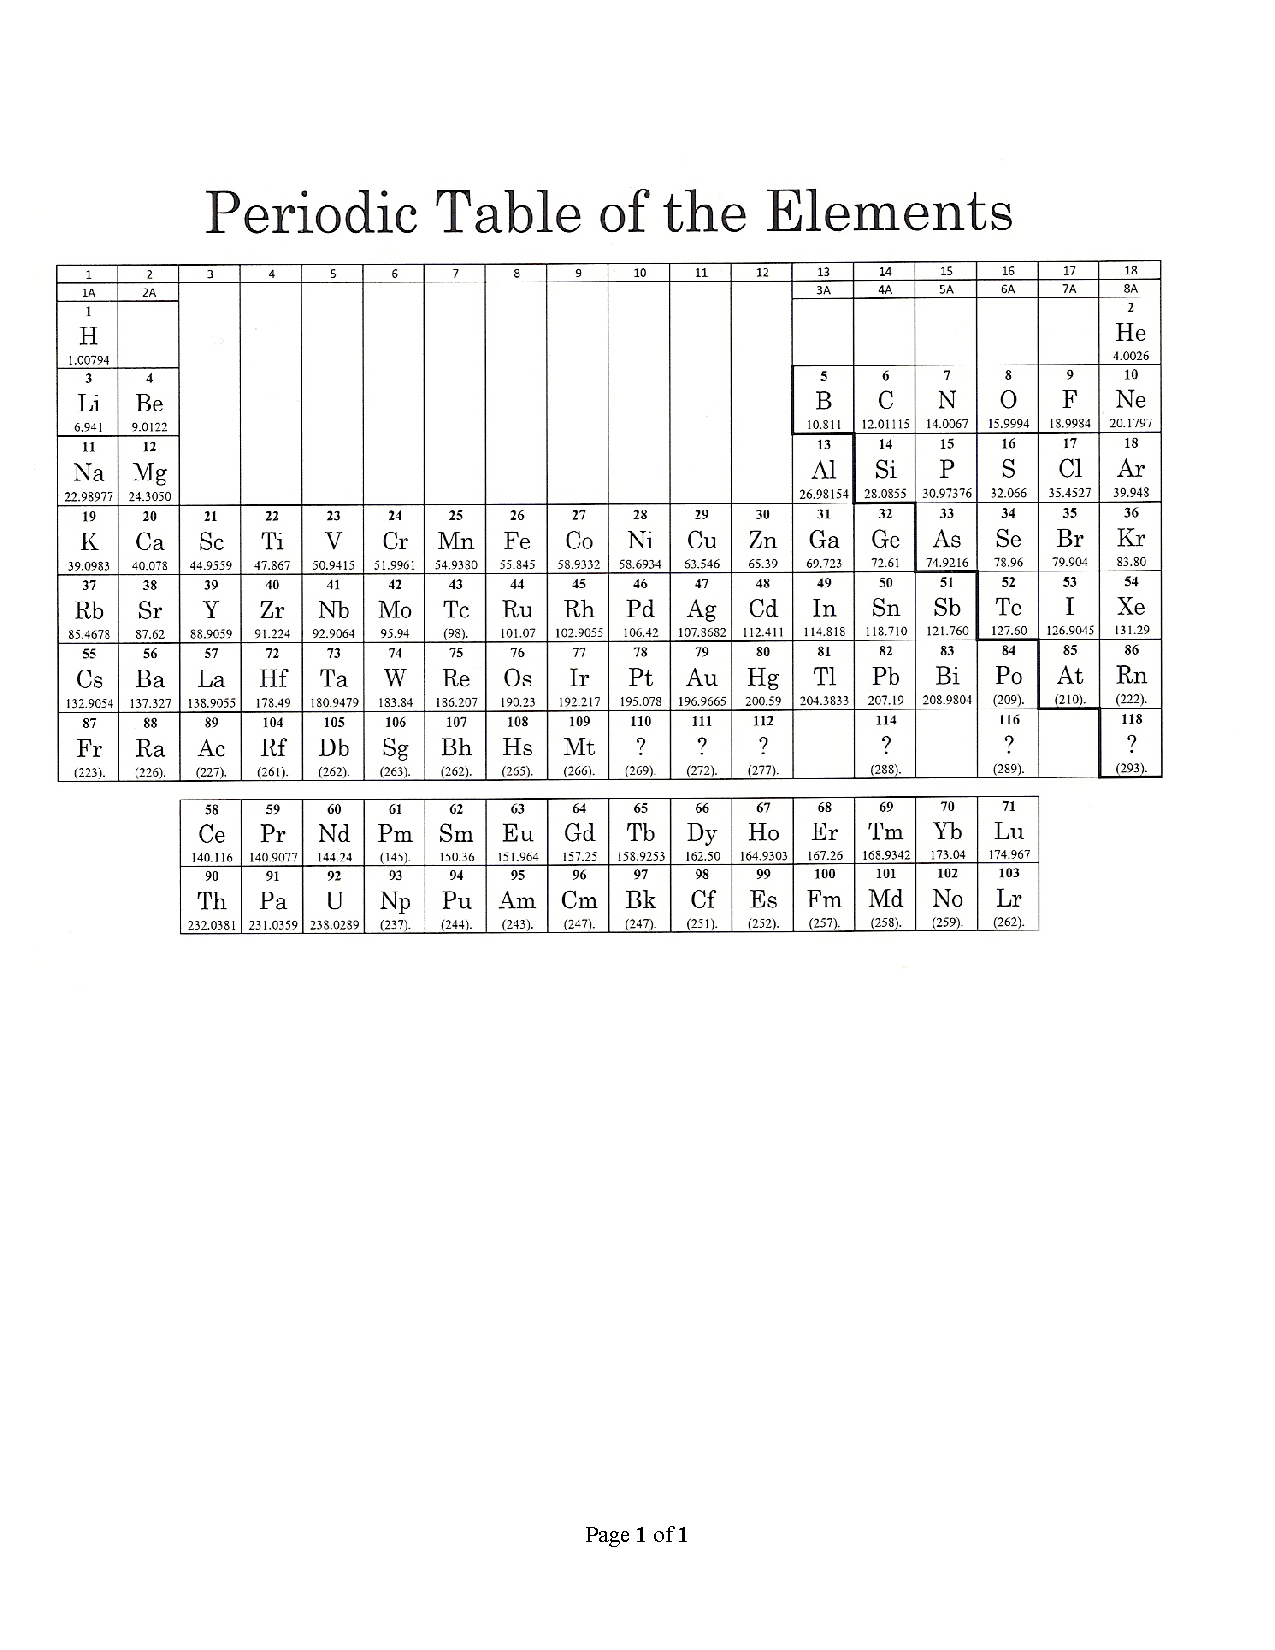
\includepdf[pages={-}]{Periodic Table for testing.pdf}

\end{document}